\documentclass[12pt,english]{article}
\usepackage{amsmath}
\usepackage{graphicx}
\usepackage{natbib}
\usepackage{booktabs}
\usepackage{parskip}

\title{Extending the SSP scenarios beyond 2100}
\author{James Rising}
\date{\today}

\begin{document}

\maketitle

The following text is modified from the supplemental information
descriptions in \citet{dietz2021tipping} and
\citet{kikstra2021tipping}.

To estimate population and income levels past 2100 along the SSP
scenarios, we fit a model to the available pre-2100 SSP scenario data
and use the fitted model to extrapolate. The same model is applied to
both income and population and is defined in terms of growth
rates. The model postulates that changes in pre-2100 income and
population growth rates are explained by a rate of convergence and a
rate of decay.

The model is as follows:
\begin{equation}\label{eq:SSP_growth}
    \text{Growth}_{it} = (1 - \beta - \delta) \text{Growth}_{i,t-1} + \delta \text{MeanGrowth}_{t-1},
  \end{equation}
  where $i$ indexes the region, $t$ indexes years, $\delta$ is the rate of convergence, $\beta$ is the decay rate and
\begin{equation}
    \text{MeanGrowth}_{t-1} = \sum_i \frac{\text{Population}_{i, 2015}}{\sum_j \text{Population}_{j, 2015}} \text{Growth}_{i,t-1}.
\end{equation}
Below, we write this as $\text{Growth}_{\cdot, t-1} \cdot w$, where $w$ is the vector of global population shares for each country.

SSP data are not available in every year, so fitting Eq.\ \eqref{eq:SSP_growth} requires a model with dynamics. We use a two-step approach, fitting the model using Stan, a computational Bayes system. The first step uses the available data directly, fitting
\begin{equation}
    \text{Growth}_{is} \sim \mathcal{N}\left( [1 - \Delta t (\beta + \delta)] \text{Growth}_{i, s-1} + \Delta t \delta \text{MeanGrowth}_{s-1}, \sigma_i\right),
\end{equation}
where $s$ is a time step, $\Delta t$ is the number of years between
time steps, and country $i$ has uncertainty $\sigma_i$. We apply a
prior that both $\beta$ and $\delta$ are between 0 and 0.5.

Next, we fit the full model, using the results of the simplified model to improve the Bayesian model convergence. In this case, for a given Markov chain Monte Carlo draw of $\beta$ and $\delta$, we calculate the entire time series:
\begin{equation}
    \widehat{\text{Growth}}_{it} \sim \mathcal{N}\left((1 - \beta - \delta) \widehat{\text{Growth}}_{i,t-1} + \delta \left[\widehat{\text{Growth}}_{\cdot, t-1} \cdot w_\cdot\right], \sigma_i\right)
\end{equation}
starting with $\widehat{\text{Growth}}_{i, 2015}$ as reported in the SSP dataset.

The probability evaluation is over both the performance of the fit and the priors:
\begin{align*}
  \text{Growth}_{is} &\sim \mathcal{N}\left(\widehat{\text{Growth}}_{i,t(s)}, \sigma_i\right)\\
\beta &\sim \mathcal{N}\left(\mu_\beta, \sigma_\beta\right) \\
\delta &\sim \mathcal{N}\left(\mu_\delta, \sigma_\delta\right) \\
\log{\sigma_i} &\sim \mathcal{N}\left(\mu_{\sigma,i}, \sigma_{\sigma,i}\right)\\
\end{align*}
where $\mu_\cdot$ is the mean estimate for the corresponding
parameter, and $\sigma_\cdot$ is the standard deviation across its
uncertainty. The prior for $\sigma_i$ is defined as a log-normal,
centered on the mean of the estimates of log $\sigma_i$.

The estimates for each SSP are shown in Table
\ref{tab:SSPs_after_2100}, with visualizations of timeseries data for SSP2 and SSP5 in Figure \ref{fig:sspextend}.

\begin{table}[h!]
    \caption{Estimated convergence and decay rates for extrapolation of growth of GDP per capita and population in the SSP socio-economic scenarios beyond 2100}
    \label{tab:SSPs_after_2100}
    \centering
   \begin{tabular}{cccc}
\toprule
SSP & Variable & $\delta$ & $\beta$ \\
\midrule
1 &   GDP per capita & 0.006205028 & 0.005930520 \\
1 &     Population & 0.008967453 & 0.005215835 \\
2 &   GDP per capita & 0.004190444 & 0.007228942 \\
2 &     Population & 0.001276993 & 0.011064426 \\
3 &   GDP per capita & 0.006273030 & 0.009597363 \\
3 &     Population & 0.001064697 & 0.007688331 \\
4 &   GDP per capita & 0.006895296 & 0.009651277 \\
4 &     Population & 0.001867587 & 0.003461600 \\
5 &   GDP per capita & 0.007766807 & 0.003843256 \\
5 &     Population & 0.003470952 & 0.004305310 \\
\bottomrule
\end{tabular}
\end{table}

\begin{figure}[h!]
    \centering
    \begin{tabular}{cc}
        \multicolumn{2}{c}{\bf Extended SSP 2} \\
        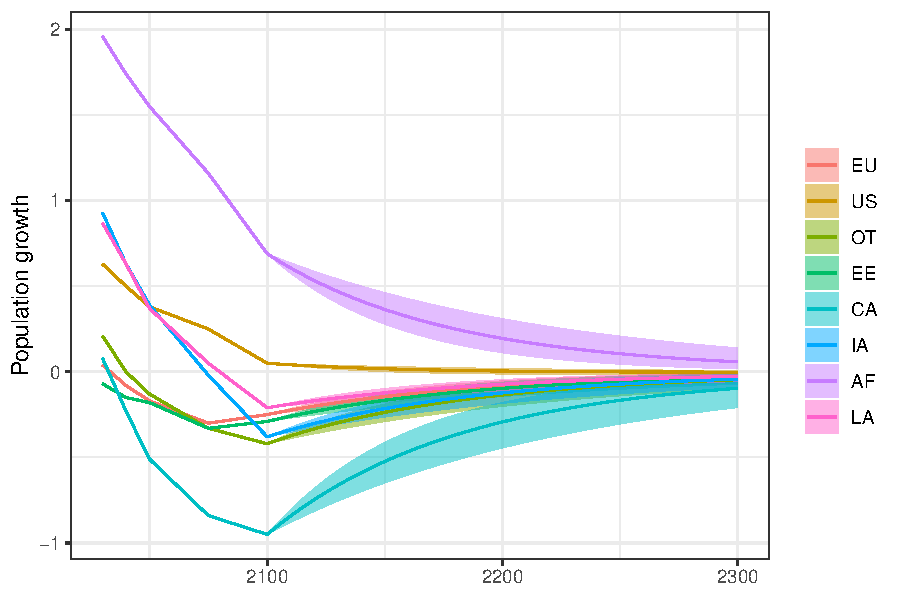
\includegraphics[width=.5\textwidth]{figures/ssp2-pop.pdf} & 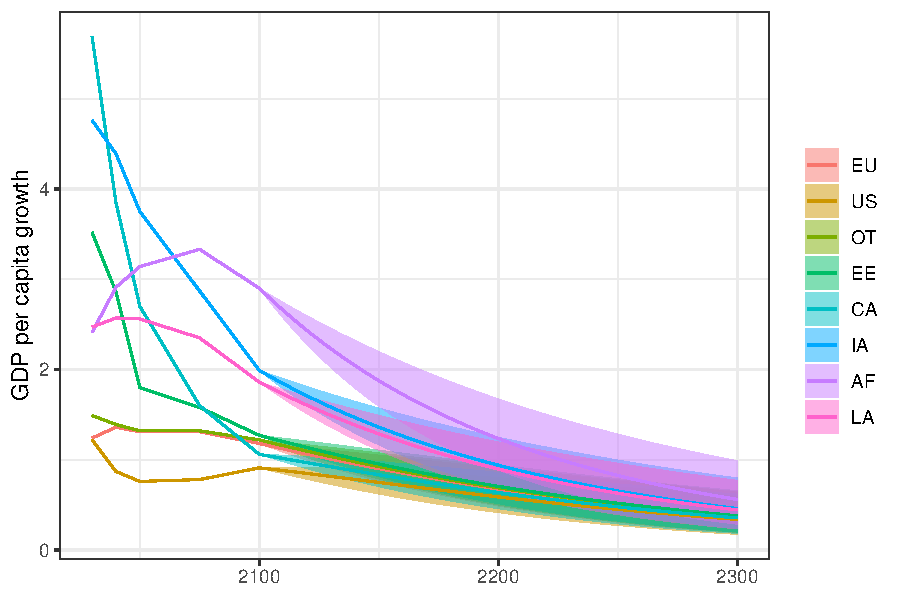
\includegraphics[width=.5\textwidth]{figures/ssp2-gdppc.pdf} \\
        \multicolumn{2}{c}{\bf Extended SSP 5} \\
        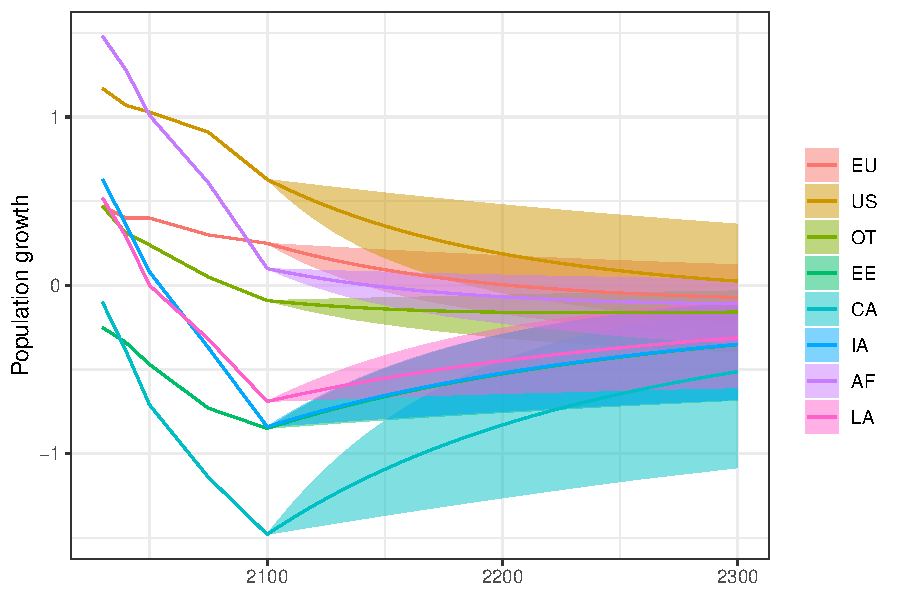
\includegraphics[width=.5\textwidth]{figures/ssp5-pop.pdf} & 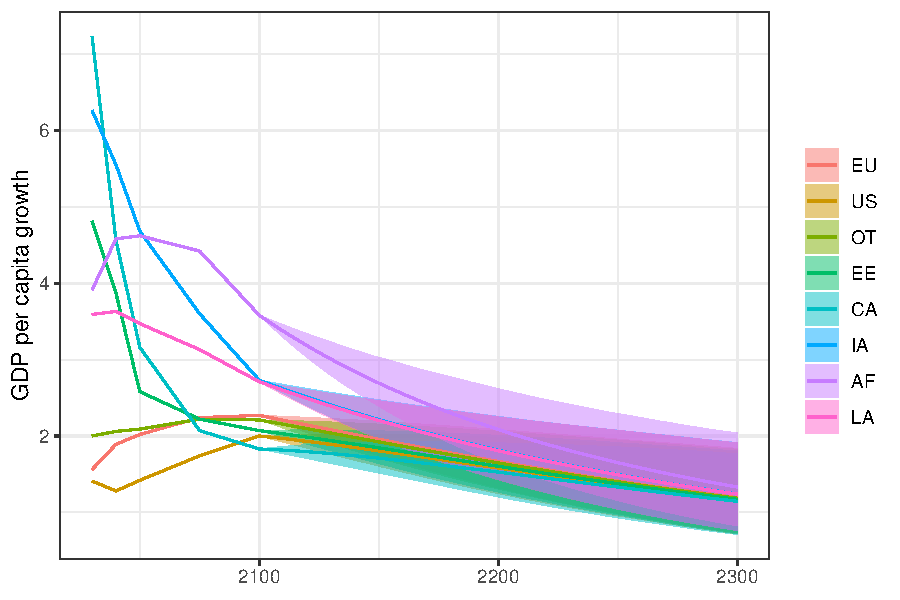
\includegraphics[width=.5\textwidth]{figures/ssp5-gdppc.pdf} \\
    \end{tabular}
    \caption{Extended SSP population and per capita GDP for SSP 2 and SSP 5. Shaded areas show 95\% credible intervals. \label{fig:sspextend}}
\end{figure}

\bibliographystyle{plainnat}
\bibliography{refs.bib}

\end{document}